% Originally generated by gen/build_ch2.py; hand-edited since 19 Oct 2026 (placeholder dashes removed).
\providecommand{\cmY}{$\checkmark$}
\providecommand{\cmN}{$\times$}
\chapter[LITERATURE REVIEW]{Literature Review}
\label{ch:literature-review}

\section{Introduction}
\label{sec:lr-introduction}

This chapter reviews the literature on which a contactless, multi-sensor
approach to corrosion detection would be built. It proceeds in six parts.
Section~\ref{sec:lr-corrosion} reviews the forms corrosion takes, where they
occur and what drives them, and so establishes what an inspection method must
find. Section~\ref{sec:lr-corrosion-detection} examines how corrosion is
currently sensed and detected, and how its severity is reported.
Section~\ref{sec:lr-detection} surveys deep learning object detection, the
family of methods that would localize corroded regions, together with the
network architectures and other artificial intelligence methods that support it.
Section~\ref{sec:lr-modalities} compares what each sensing modality can
contribute to a corrosion inspection, and Section~\ref{sec:lr-fusion} reviews
how modalities are combined, at what level, and with what effect.
Section~\ref{sec:lr-gap} brings these strands together into a statement of the
research gap.

Each body of literature is summarized in a comparison table that records, for
every study, the type of data used, the method, the application, and the
advantages and limitations reported by its authors. For object detection and
sensor fusion, two tables are given: a method-focused table that records what
each algorithm achieves, and a data-focused table that records what each sensing
modality contributes and where it falls short. All counts quoted in the text are
taken from these tables, with one study counted per reference. The comparison
tables include journal articles published from 2020 to 2026, with one exception:
an earlier deep learning detector of hull plate corrosion \citep{Yao2019} is retained as
an early example of learned corrosion detection on marine steel. Conference papers are cited in the text, outside
the tables, where they report evidence not available in the journal literature
\citep{Soares2023,Ding2025,Zheng2025,Haitz2022,Mota2024}.

Much of the fusion literature reviewed in Section~\ref{sec:lr-fusion} comes from
autonomous driving, surveillance and image fusion rather than from corrosion.
This is deliberate. Multi-sensor fusion matured in those fields, and the
registration methods, fusion architectures and evaluation practices developed
there are what a corrosion application would have to draw on. How little of that
work has reached corrosion inspection is itself part of the gap stated in
Section~\ref{sec:lr-gap}.

% =====================================================================
\section{Corrosion}
\label{sec:lr-corrosion}

\subsection{Mechanism}

Corrosion is the process by which a metal interacts with its environment and
transforms into a more stable, oxidized state \citep{Elizalde2023}. It proceeds through
electrochemical interactions between the metal surface and a corrosive
environment containing oxygen, moisture or aggressive chemicals \citep{Alvani2026}. On steel,
the anodic reaction dissolves iron into ferrous ions, which are further oxidized
and hydrolyzed to form iron hydroxides and oxides, releasing hydrogen ions in the
process \citep{Liu2026}.

Pitting is the localized form of this process. It begins where the protective
oxide film breaks down; the exposed metal then dissolves, and the hydrolysis of
the dissolved metal ions acidifies the solution inside the pit \citep{Liu2026}. Localized
acidification, the enrichment of cations and the restricted diffusion of species
out of the pit together make conditions inside the pit progressively more
corrosive, so that pitting becomes autocatalytic \citep{Liu2026}. Chloride drives this
process in most of the settings reviewed. In water supply systems, chlorine
disinfectant creates a high-chloride, acidic and strongly oxidizing environment
at the pipe surface \citep{Li2022}. A rust layer over a pit can transport chloride into
the pit while preventing the aggressive pit chemistry from being diluted, which
delays or prevents repassivation and stabilizes the pit \citep{Nguyen2026}. The resulting pits
are deep wells with small diameters \citep{Soares2023}, so the visible extent of a pit says
little about how much metal has been lost beneath it.

\subsection{Forms of Corrosion and Where They Occur}

Table~\ref{tab:corrosion} summarizes the forms of corrosion examined in the
reviewed studies, the settings in which they occur, the factors that drive them
and whether each study detects the corrosion it describes.

{\scriptsize
\renewcommand{\arraystretch}{1.15}
\setlength{\tabcolsep}{3pt}
\begin{xltabular}{\textwidth}{>{\RaggedRight\arraybackslash}p{1.5cm}>{\RaggedRight\arraybackslash}p{2.6cm}>{\RaggedRight\arraybackslash}X>{\RaggedRight\arraybackslash}p{2.4cm}>{\RaggedRight\arraybackslash}p{1.9cm}}
\caption{Forms of corrosion in the reviewed studies, where they occur, what drives them and whether the study detects them}\label{tab:corrosion}\\
\toprule
\textbf{Type} & \textbf{Area of occurrence} & \textbf{Factors and how it forms} & \textbf{Detection} & \textbf{Ref.} \\
\midrule
\endfirsthead
\multicolumn{5}{@{}l}{\textit{\tablename~\thetable\ (continued)}}\\
\toprule
\textbf{Type} & \textbf{Area of occurrence} & \textbf{Factors and how it forms} & \textbf{Detection} & \textbf{Ref.} \\
\midrule
\endhead
\midrule\multicolumn{5}{r@{}}{\textit{continued on next page}}\\
\endfoot
\bottomrule
\multicolumn{5}{@{}p{\textwidth}@{}}{\textit{Note.} A blank cell repeats the entry above it.}\\
\endlastfoot
Pitting & Offshore and marine equipment & Chloride from high salinity, high temperature in the marine environment, and chemical composition of stored fluids and production water penetrate the passive film, causing localized breakdown & No & \citep{Liu2026,Wang2021,Khodabux2021,Nugroho2021} \\
 &  &  & RGB & \citep{Mao2026} \\
 & Oil and gas pipelines (buried and above ground) & Corrosive fluids/soil/seawater and acidic environments cause chemical/electrochemical reactions, often intensified by physical stress. & No & \citep{Arzaghi2020,Akhlaghi2023} \\
 &  &  & RGB & \citep{Malashin2024} \\
 &  &  & Ultrasonic (UT) & \citep{Huang2026a} \\
 & Water supply and treatment systems & Chloride from NaClO disinfectant penetrates the passive film, initiating corrosion; susceptibility depends on chloride concentration and film stability/composition. & No & \citep{Li2022,Nguyen2026} \\
 &  & Iron contamination, water content, and chloride concentration promote pit initiation, while the rust layer allows chloride ingress and traps metal ions, stabilizing the aggressive pit environment. &  &  \\
 &  &  & Thermal & \citep{Liu2021} \\
 & Electrical power systems & Anodic polarization breaks down the passive film, causing metal oxidation and dissolution that initiates pit formation & No & \citep{Wojciechowski2025} \\
 & Buildings & Metals interact with their environment and transform into a more stable oxidized state & Thermal & \citep{Elizalde2023} \\
 &  & High rare earth (RE) segregation in Mg alloys creates RE rich zones which are anodic in nature and cause localized pitting & No & \citep{Qin2026} \\
 &  & Immersion in HCl solution produces surface corrosion & Multi-spectral imaging & \citep{Egodawela2025} \\
 & Brackish-water drainage channels & Chloride from brackish water and repeated wetting and drying break down the steel's protective passive film, starting pits & RGB & \citep{Suzuki2026} \\
 & Offshore wind structures (North Sea) & Chlorine ions in seawater keep pits growing once they start; near the seabed, nitrogen, which boosts marine growth, led to more and deeper pits & Grayscale scans (paper rubbings) + pit gauge & \citep{Khodabux2021a} \\
\midrule
Uniform & Offshore wind turbines & Seawater temperature, dissolved oxygen and salinity change with depth, so the corrosion rate varies from the splash zone to the seabed & No & \citep{Khodabux2020} \\
 & Oil and gas infrastructure & Environmental exposure, electrochemical reactions, and fluctuating operating conditions cause pipe-wall thinning and mechanical degradation. & Acoustic signals & \citep{Yang2026a} \\
 & Reinforced concrete buildings & Chloride invasion and concrete carbonization destroys the passivation film of the rebar, leading to corrosion. High chloride ion concentration, and high humidity accelerates the process. & Pulsed eddy current & \citep{Yang2025} \\
\midrule
Atmospheric & Industrial infrastructure & Continuous sodium chloride exposure drives corrosion in steel & Infrared & \citep{DeKerf2022} \\
\midrule
Microbial & Offshore engineering equipment & Corrosion occurs due to the presence of corrosive media e.g., chloride ions, oxygen, water and sulfate reducing bacteria (SRB) & No & \citep{Liang2021} \\
\end{xltabular}
}


\begin{figure}[htbp]
\centering
\begin{subfigure}[b]{0.56\textwidth}\centering
\includegraphics[width=\linewidth]{nugroho2021_fig5.jpg}
\caption{Pitting: laser scan of a pitted specimen}
\end{subfigure}\hfill
\begin{subfigure}[b]{0.40\textwidth}\centering
\includegraphics[width=\linewidth]{khodabux2020_coupon.jpg}
\caption{Uniform: coupon after sea exposure}
\end{subfigure}\\[6pt]
\begin{subfigure}[b]{0.52\textwidth}\centering
\includegraphics[width=\linewidth]{dekerf2022_fig1.jpg}
\caption{Atmospheric: steel after salt-spray testing}
\end{subfigure}\hfill
\begin{subfigure}[b]{0.44\textwidth}\centering
\includegraphics[width=\linewidth]{liang2021_fig10a2.jpg}
\caption{Microbial: bacteria on bare steel}
\end{subfigure}
\caption[Forms of corrosion examined in the reviewed studies]{Forms of corrosion examined in the reviewed studies. (a)~3D laser scan of corroded
ballast-tank steel, reproduced from \citet{Nugroho2021}, Fig.~5; (b)~steel coupon from
the North Sea, reproduced from \citet{Khodabux2020}; (c)~carbon steel after an accelerated
salt-spray test, reproduced from \citet{DeKerf2022}, Fig.~1; (d)~fluorescence image of
sulfate-reducing bacteria on bare steel, reproduced from \citet{Liang2021}, Fig.~10(a2).}
\label{fig:corrosion-forms}
\end{figure}

Figure~\ref{fig:corrosion-forms} shows four of these forms as they appear in the
reviewed studies. Three findings emerge from Table~\ref{tab:corrosion}. First, pitting dominates:
it is the subject of 18 of the 23 studies, against three on uniform corrosion
\citep{Khodabux2020,Yang2025,Yang2026a} and one each on atmospheric \citep{DeKerf2022} and microbial corrosion \citep{Liang2021}.
Second, pitting is concentrated in chloride-rich settings. Seven of the 18
pitting studies concern marine, offshore or brackish-water environments
\citep{Liu2026,Wang2021,Khodabux2021,Nugroho2021,Mao2026,Khodabux2021a,Suzuki2026}, four concern oil and gas pipelines
\citep{Akhlaghi2023,Arzaghi2020,Malashin2024,Huang2026a}, three concern water supply systems \citep{Li2022,Nguyen2026,Liu2021}, three concern
buildings \citep{Elizalde2023,Qin2026,Egodawela2025} and one concerns electrical power systems \citep{Wojciechowski2025}.
Chloride is named as a driver of pitting in the marine, water supply and
drainage settings alike \citep{Liu2026,Li2022,Nguyen2026,Suzuki2026,Khodabux2021a}. Third, only 11 of the 23 studies
attempt to detect corrosion at all. Of these, three use RGB images
\citep{Malashin2024,Mao2026,Suzuki2026}, two use thermal imaging \citep{Elizalde2023,Liu2021}, and one each uses ultrasonic
testing \citep{Huang2026a}, multispectral imaging \citep{Egodawela2025}, shortwave infrared
hyperspectral imaging \citep{DeKerf2022}, acoustic signals \citep{Yang2026a}, pulsed eddy current
\citep{Yang2025} and scanned paper rubbings measured with a pit gauge \citep{Khodabux2021a}. The remaining
12 studies model how pits form, predict their growth or test means of preventing
them \citep{Liu2026,Li2022,Nguyen2026,Wang2021,Qin2026,Akhlaghi2023,Wojciechowski2025,Khodabux2020,Liang2021,Khodabux2021,Nugroho2021,Arzaghi2020}.

For inspection, the implication is that the form of corrosion that matters most
is also the one that is hardest to see. Because pits are deep and narrow with
small openings \citep{Soares2023}, an inspection that reports only the visible area of a
corroded region can understate the damage. Pit depth and metal loss must be
measured, not only area.

% =====================================================================
\section{Corrosion Inspection and Detection}
\label{sec:lr-corrosion-detection}

\subsection{Sensing in Corrosion Detection Studies}

In practice, corrosion is still widely found by visual inspection, which is
subjective and inconsistent between inspectors and conditions \citep{Espinoza2026,Savino2025}. Table~\ref{tab:corrosion-detection} summarizes the studies
that detect corrosion, the settings they address and the sensing data they use.

{\scriptsize
\renewcommand{\arraystretch}{1.15}
\setlength{\tabcolsep}{3pt}
\begin{xltabular}{\textwidth}{>{\RaggedRight\arraybackslash}p{3.6cm}>{\RaggedRight\arraybackslash}X>{\RaggedRight\arraybackslash}p{4.2cm}}
\caption{Corrosion detection studies: setting and sensing data}\label{tab:corrosion-detection}\\
\toprule
\textbf{Area of occurrence} & \textbf{Detection data} & \textbf{Ref.} \\
\midrule
\endfirsthead
\multicolumn{3}{@{}l}{\textit{\tablename~\thetable\ (continued)}}\\
\toprule
\textbf{Area of occurrence} & \textbf{Detection data} & \textbf{Ref.} \\
\midrule
\endhead
\midrule\multicolumn{3}{r@{}}{\textit{continued on next page}}\\
\endfoot
\bottomrule
\multicolumn{3}{@{}p{\textwidth}@{}}{\textit{Note.} A blank cell repeats the entry above it. \citet{Lavadiya2022} names no setting and is discussed in the text.}\\
\endlastfoot
Marine environments & Hyperspectral and multispectral imaging & \citep{Hernndez-Surez2026} \\
 & Hyperspectral imaging & \citep{Arias2025} \\
 & RGB & \citep{Fu2024,Imran2025,Yao2019,Hu2023} \\
 & LiDAR, hyperspectral and RGB & \citep{PallasEnguita2025} \\
\midrule
Oil and gas infrastructure & RGB & \citep{Alvani2026} \\
\midrule
Civil infrastructure & Ground-penetrating radar (radargrams) & \citep{Bui2026} \\
 & RGB & \citep{Savino2025,Maharjan2025} \\
\midrule
Industrial environments & RGB & \citep{Espinoza2026,Nash2022} \\
 & Thermal imaging & \citep{Doshvarpassand2022} \\
\end{xltabular}
}


Where these studies name a cause of corrosion, it is exposure to seawater, salt
and humidity in marine settings
\citep{Hernndez-Surez2026,Arias2025,Fu2024,Imran2025,PallasEnguita2025}, the loss
of a coating that exposes the metal to oxygen and water \citep{Hu2023}, oxygen,
moisture and aggressive chemicals in oil and gas infrastructure \citep{Alvani2026},
the ingress of oxygen, moisture and chlorides into civil structures \citep{Bui2026},
water running down the steel \citep{Savino2025}, and acid, salt or sulfate
exposure \citep{Lavadiya2022}.

Taking every reviewed study that senses or detects corrosion, from
Tables~\ref{tab:corrosion} and~\ref{tab:corrosion-detection} and from the
corrosion rows of the detection and fusion tables in
Sections~\ref{sec:lr-detection} and~\ref{sec:lr-fusion}, gives 33 studies. Of
these, 16 rely on RGB images alone
\citep{Malashin2024,Mao2026,Espinoza2026,Fu2024,Alvani2026,Imran2025,Yao2019,Nash2022,Savino2025,Maharjan2025,Li2024b,Suzuki2026,Rahman2021,Hu2023,Yu2023,HerndonTien2025}.
Five use hyperspectral or multispectral imaging \citep{Egodawela2025,DeKerf2022,Arias2025,Lavadiya2022,Hernndez-Surez2026}, three use
thermal imaging alone \citep{Elizalde2023,Doshvarpassand2022,Liu2021} and four use another single sensor: pulsed
eddy current \citep{Yang2025}, acoustic signals \citep{Yang2026a}, ground-penetrating radar \citep{Bui2026} and
scanned rubbings \citep{Khodabux2021a}. Only five combine more than one sensor (Figure~\ref{fig:corr-sensing}):
ultrasonic and field signature probes \citep{Huang2026a}; RGB with active thermography
\citep{Lim2021}; RGB with LiDAR \citep{Maru2025,PimenteldeFigueiredo2025}; and LiDAR with hyperspectral imaging
\citep{PallasEnguita2025}. Of these five, only one adds thermal imaging \citep{Lim2021}, and none combines
RGB, thermal and LiDAR data. Three conference papers, outside the tables, also
combine sensors for corrosion: ultrasonic guided waves with RGB images and a
point cloud \citep{Ding2025}, 3D laser scanning with RGB, ultrasonic thickness measurement
and magnetic flux leakage \citep{Zheng2025}, and RGB with laser triangulation \citep{Haitz2022}.
None of them uses thermal imaging.


\begin{figure}[htbp]
\centering
\begin{tikzpicture}
\begin{axis}[
  xbar, bar width=0.48cm, width=0.78\textwidth, height=5.4cm,
  xmin=0, xmax=18.5, xtick={0,4,8,12,16},
  symbolic y coords={Multi-sensor,Other single sensor,Thermal only,Spectral only,RGB only},
  ytick={Multi-sensor,Other single sensor,Thermal only,Spectral only,RGB only}, y tick label style={font=\small}, x tick label style={font=\small},
  xlabel={Number of studies (of 33)}, xlabel style={font=\small},
  axis x line*=bottom, axis y line*=left, enlarge y limits=0.14,
  xmajorgrids, grid style={black!12},
  nodes near coords, nodes near coords align={horizontal},
  every node near coord/.append style={font=\small, text=black},
]
\addplot[bar shift=0pt, fill=chartBlue, draw=none] coordinates {(16,RGB only) (5,Spectral only) (3,Thermal only) (4,Other single sensor)};
\addplot[bar shift=0pt, fill=chartOrange, draw=none] coordinates {(5,Multi-sensor)};
\end{axis}
\end{tikzpicture}
\caption[Sensing used in the reviewed corrosion studies]{Sensing used in the 33 corrosion-sensing studies reviewed. Only five
combine sensors, and only one of those adds thermal imaging \citep{Lim2021}.}
\label{fig:corr-sensing}
\end{figure}

\subsection{What Each Approach Recovers}

RGB-based detection relies on the color and texture of rust. Corrosion on steel
shows a rough texture and a well-defined red or red-brown color \citep{Rahman2021,HerndonTien2025}, and
color separates rust from bare metal and surface oil that look alike in
grayscale \citep{Hu2023}. The same reliance on color is the source of its failures.
Detection degrades with lighting and viewing angle \citep{Hu2023,Yu2023,HerndonTien2025}; branches,
wires and insect hives mimic corrosion in texture and color \citep{HerndonTien2025}; areas of
water are misclassified as corrosion \citep{Rahman2021}; and severity grading by eye remains
subjective \citep{Li2024b}. Above all, an image shows only the surface opening of a pit,
so its depth is difficult to judge \citep{Suzuki2026}.

Spectral imaging addresses the confusion between rust and its look-alikes.
Hyperspectral data separate coated from corroded material even where their RGB
values are similar \citep{PallasEnguita2025} (Figure~\ref{fig:multisensor}b,c). They have been used to assess marine steel
corrosion \citep{Arias2025}, to remove visual ambiguity and identify sources of corrosion
\citep{Lavadiya2022}, and to detect corrosion with a few selected bands \citep{Hernndez-Surez2026}. Their cost and bulk, however, limit
their use in the field \citep{Tang2025}, and hyperspectral sensors exceed the payload of
compact drones \citep{PallasEnguita2025}.

Thermal imaging responds to what lies beneath the surface rather than to its
color. Active infrared thermography improves the detection of hidden corrosion
under paint on metal sheets \citep{Elizalde2023}, cold thermography approximates the depth of
subsurface defects \citep{Doshvarpassand2022}, and deep networks have quantified pitting from
thermographic data \citep{Liu2021}. On steel bridges, fusing RGB with active thermography
revealed corrosion beneath the coating that was invisible in RGB images \citep{Lim2021}.

Geometric sensing measures the surface itself. LiDAR fused with RGB images has
detected and measured section loss in steel members \citep{Maru2025} and mapped corrosion
in an industrial plant with a portable, handheld rig \citep{PimenteldeFigueiredo2025} (Figure~\ref{fig:multisensor}a); laser triangulation
has been added to RGB to form a five-dimensional feature space for corrosion
detection on industrial objects \citep{Haitz2022}; and LiDAR has been combined with
hyperspectral imaging for ballast tank inspection \citep{PallasEnguita2025}. These studies show
that geometry can be recovered without contact, but they are limited to
laboratory specimens \citep{Maru2025,PallasEnguita2025} or are sensitive to position drift \citep{PimenteldeFigueiredo2025}.


\begin{figure}[htbp]
\centering
\begin{subfigure}[b]{0.40\textwidth}\centering
\includegraphics[width=\linewidth]{pimentel2025_fig11a.jpg}
\caption{Handheld LiDAR and RGB rig}
\end{subfigure}\hfill
\begin{minipage}[b]{0.57\textwidth}\centering
\begin{subfigure}[b]{\linewidth}\centering
\includegraphics[width=\linewidth]{pallas2025_fig3.jpg}
\caption{RGB photograph of a partly coated beam}
\end{subfigure}\\[8pt]
\begin{subfigure}[b]{\linewidth}\centering
\includegraphics[width=\linewidth]{pallas2025_fig5.jpg}
\caption{Hyperspectral heatmap of the same beam}
\end{subfigure}
\end{minipage}
\caption[Multi-sensor corrosion set-ups from the reviewed studies]{Multi-sensor corrosion set-ups from the reviewed studies. (a)~Operator
carrying a handheld LiDAR and RGB camera with a computing backpack, used to map
corrosion in an industrial plant, reproduced from \citet{PimenteldeFigueiredo2025},
Fig.~11a. (b)~A steel beam with coating on top and rust below and (c)~its
hyperspectral heatmap (690--840~nm), in which coating (red) and rust (blue)
separate, reproduced from \citet{PallasEnguita2025}, Figs.~3 and~5.}
\label{fig:multisensor}
\end{figure}

Where metal loss is quantified in the reviewed studies, it is measured by contact
or on laboratory specimens. Wall thickness is measured with ultrasonic and field
signature probes \citep{Huang2026a} or with handheld ultrasonic and magnetic flux leakage
equipment \citep{Zheng2025}; pit depth is measured by hand with a pit gauge \citep{Khodabux2021a}; and
thermographic and multispectral depth estimates are obtained on laboratory
specimens \citep{Doshvarpassand2022,Liu2021,Egodawela2025}, as is the LiDAR-based section loss of \citep{Maru2025}.

\subsection{Reporting of Severity}

Of the 37 reviewed corrosion studies, 20 report a measure of severity, listed in
Table~\ref{tab:severity}.

{\scriptsize
\renewcommand{\arraystretch}{1.15}
\setlength{\tabcolsep}{3pt}
\begin{xltabular}{\textwidth}{p{1.0cm}>{\RaggedRight\arraybackslash}Xp{1.0cm}>{\RaggedRight\arraybackslash}X}
\caption{Severity measures reported by the reviewed corrosion studies}\label{tab:severity}\\
\toprule
\textbf{Ref.} & \textbf{Severity reported} & \textbf{Ref.} & \textbf{Severity reported} \\
\midrule
\endfirsthead
\multicolumn{4}{@{}l}{\textit{\tablename~\thetable\ (continued)}}\\
\toprule
\textbf{Ref.} & \textbf{Severity reported} & \textbf{Ref.} & \textbf{Severity reported} \\
\midrule
\endhead
\midrule\multicolumn{4}{r@{}}{\textit{continued on next page}}\\
\endfoot
\bottomrule
\endlastfoot
\citep{Liu2026} & Pit depth of up to 3.7~mm, width up to 18~mm & \citep{Hu2023} & Share of the buoy's metal that is rusted, converted to a rust grade \\
\citep{Wang2021} & Pit depth increases with depth of sea level (4.68 to 10.86~$\mu$m) & \citep{Bui2026} & Graded in four levels, negligible to severe \\
\citep{Qin2026} & Max pit depth of about 1.3~mm & \citep{Hernndez-Surez2026} & Graded 1 to 3 by exposure time \\
\citep{Egodawela2025} & Measured by depth of corrosion pits (up to 5~mm) & \citep{Rahman2021} & Graded heavy, medium or light \\
\citep{Akhlaghi2023} & Pit depth 0.41 to 13.44~mm in field data & \citep{Arias2025} & Loss of structural integrity; reduction of cross sectional area; graded in five classes, none to severe \\
\citep{Huang2026a} & Pit depth can be $>$ half the pipe wall thickness & \citep{Fu2024} & Graded light, moderate or heavy \\
\citep{Khodabux2021a} & Max pit depth of 1.05~mm after 111 days & \citep{Malashin2024} & Binary classification (corroded vs. non-corroded) \\
\citep{Yang2025} & Rebar diameter falls 18~mm to 10.58~mm (41.22\% cross section loss ratio) & \citep{Elizalde2023} & Material loss; loss of mechanical quality \\
\citep{Savino2025} & Corroded area of up to 0.046 m$^2$ & \citep{Wojciechowski2025} & Reduction in lifespan of electrochemical capacitors (ECs) \\
\citep{Suzuki2026} & Pit count and share of surface pitted & \citep{Yang2026a} & Thin pipe walls, mechanical degradation, structural failure \\
\end{xltabular}
}


The other 17 report no measure of severity
\citep{Li2022,Nash2022,Nguyen2026,Doshvarpassand2022,Lavadiya2022,Maharjan2025,Mao2026,PallasEnguita2025,Khodabux2020,Yu2023,HerndonTien2025,DeKerf2022,Liang2021,Espinoza2026,Alvani2026,Imran2025,Yao2019}.
The 20 that do use measures that cannot be compared with one another: pit depth
or metal loss in eight \citep{Liu2026,Wang2021,Qin2026,Egodawela2025,Akhlaghi2023,Huang2026a,Khodabux2021a,Yang2025}, corroded area or
the share of the surface affected in three \citep{Savino2025,Suzuki2026,Hu2023}, ordinal grades
or a binary label in six \citep{Bui2026,Hernndez-Surez2026,Rahman2021,Arias2025,Fu2024,Malashin2024}, and qualitative
consequences such as material loss or reduced service life in three
\citep{Elizalde2023,Wojciechowski2025,Yang2026a}. Camera-based studies report area or grades; depth and metal loss
come from contact measurement, modeling or laboratory work. No reviewed study
estimates both the corroded area and the metal loss of a detected region from
contactless field data.

\subsection{Data Availability}

Data are a recurring constraint. The RGB-thermal images of the bridge study were
withheld under a confidentiality agreement with the bridge authority \citep{Lim2021}, and
the data of a recent dual-modal corrosion network are available only on request
\citep{Mao2026}. Public corrosion datasets do exist, such as the Rust-Seg-2 set used by
\citep{Espinoza2026}, but they contain RGB images only. No public dataset pairs RGB, thermal
and LiDAR data of corroded surfaces.

% =====================================================================
\section{Object Detection}
\label{sec:lr-detection}

\subsection{Detection Methods and Data}

Object detection locates each object of interest in an image with a bounding box
and a class label. Tables~\ref{tab:detection-method} and~\ref{tab:detection-data}
summarize the 40 detection studies reviewed, the first by method and the second
by the type of data used.

{\scriptsize
\renewcommand{\arraystretch}{1.15}
\setlength{\tabcolsep}{3pt}
\begin{xltabular}{\textwidth}{>{\RaggedRight\arraybackslash}p{1.6cm}>{\RaggedRight\arraybackslash}p{2.2cm}>{\RaggedRight\arraybackslash}p{2.3cm}>{\RaggedRight\arraybackslash}X>{\RaggedRight\arraybackslash}Xp{0.95cm}}
\caption{Object detection studies: methods, applications, and the advantages and limitations of each method}\label{tab:detection-method}\\
\toprule
\textbf{Type of data} & \textbf{Method} & \textbf{Application} & \textbf{Advantages} & \textbf{Limitations} & \textbf{Ref.} \\
\midrule
\endfirsthead
\multicolumn{6}{@{}l}{\textit{\tablename~\thetable\ (continued)}}\\
\toprule
\textbf{Type of data} & \textbf{Method} & \textbf{Application} & \textbf{Advantages} & \textbf{Limitations} & \textbf{Ref.} \\
\midrule
\endhead
\midrule\multicolumn{6}{r@{}}{\textit{continued on next page}}\\
\endfoot
\bottomrule
\multicolumn{6}{@{}p{\textwidth}@{}}{\textit{Note.} A blank cell repeats the entry above it. \citet{Gong2022} reports no limitation of its method and appears in Table~\ref{tab:detection-data} only.}\\
\endlastfoot
RGB & CNN (Faster R-CNN, YOLOv3 to YOLOv11, SSD, FCOS, RetinaNet, ResNet, U-ShapeNet, BI-CNN) & Detecting remote sensing targets (multi-scale, small) & Two-stream shrinking keeps fine detail & Slower than standard light YOLO models & \citep{Wang2026a} \\
 &  &  & Better feature extraction, and hence object detection in RSI & Poor detection of small objects with unclear boundaries & \citep{Zhang2024} \\
 &  &  & Tuned learning loss lifts accuracy & Tested on one dataset (DOTA) only & \citep{Lalitha2022} \\
 &  & Detecting objects in low light & Improved object detection in low light conditions & No gain on medium-sized objects & \citep{Wu2023} \\
 &  & Detecting everyday objects & Fewer false detections and better recall & Misses some blocked objects & \citep{Wu2026} \\
 &  &  & YOLOv3 fastest, great results overall & Struggles with small targets & \citep{Srivastava2021} \\
 &  & Detecting boiler wall defects & Shallow feature fusion finds tiny, dense defects & Attention modules add parameters, harder to train & \citep{Sun2022} \\
 &  & Detecting corroded bridge bolts & Detects corrosion and grades it into three severity levels & Corrosion grading is subjective, and no corrosion prediction & \citep{Li2024b} \\
 &  & Detecting airplanes, cars and ships & Multi-scale contextual information improves feature representation, with stable performance in deep layers & Computationally expensive, requiring 38.74 billion operations & \citep{Han2022} \\
 &  & Detecting vehicles & Fewer weights and cheaper to deploy & Not verified on real mobile hardware & \citep{Liu2026a} \\
 &  & Detecting maritime ships & Outperforms existing FPN models in precision, recall, and GIoU & Cost grows with the number of regions of interest & \citep{Mbietieu2025} \\
 &  & Detecting small flying objects & Runs at 147 FPS, good for low-altitude flying object detection & Not yet adapted to embedded devices & \citep{Tao2021} \\
 &  & Detecting small UAV targets & Enhanced feature extraction and small object detection & Model is not yet light weight enough for UAV hardware & \citep{Jiang2025} \\
 &  & Detecting tiny objects and people & Enhanced detection performance of tiny objects & Real-time speed untested & \citep{Chen2025} \\
 &  & Detecting dense aerial targets & Improved small object detection in aerial images & Model is not yet light weight enough for UAV hardware & \citep{Sun2023} \\
 &  & Detecting  small objects & Multi-view object detection approach solves the occluded object problem & Multi-stage pipeline which increases system complexity & \citep{Zheng2023} \\
 & CNN (U-Net) & Detecting corrosion & More accurate than brightness thresholding, and robust to natural lighting variation & Trained on only two images from a single site & \citep{Suzuki2026} \\
 & CNN (DeepLab) &  & Segments corrosion at pixel level instead of a bounding box, so its area can be assessed & Missed lighter corrosion; areas with water mostly misclassified as corrosion & \citep{Rahman2021} \\
 & CNN (U-Net) + Image processing &  & Segmentation more accurate than traditional and state-of-the-art methods; fewer false detections than grayscale thresholding & Data still lacking, limiting accuracy and generalization & \citep{Hu2023} \\
 & CNN (YOLO) &  & Real time on the drone's on-board computer; outperforms other state-of-the-art detectors & Bar corrosion easily mistaken for nubby corrosion, which differs only in shape & \citep{Yu2023} \\
 & CNN + K-means &  & Outperforms thresholding and deep learning; images of a new bridge need no labeling & Not yet accurate enough to be used directly in bridge inspections & \citep{HerndonTien2025} \\
\midrule
RGB (IR unfused) & Transformer & Detecting small objects & Trains quickly with very little data & Lacks variety of real environments & \citep{Zhang2026c} \\
\midrule
Grayscale scans (paper rubbings) + pit gauge & Image processing & Detecting corrosion & Extracts pit area, aspect ratio, and minor and major lengths & Pit depth measured by hand with a pit gauge, which is time-consuming & \citep{Khodabux2021a} \\
\midrule
Thermal & CNN (YOLOv8, YOLOv10) & Detecting people and vehicles & Improves detection accuracy in a lightweight model built for drone edge hardware & Not yet tested across flight altitudes, night or adverse weather, or on embedded hardware & \citep{Liu2026c} \\
 &  &  & More accurate than YOLOv8 with fewer parameters, suiting real-time use on edge devices & Still struggles with distant targets with weak thermal radiation in low-contrast scenes & \citep{Wang2024b} \\
 &  & Detecting objects & More accurate than YOLOv8 with fewer parameters & Lightweight thermal image enhancement still gives a poor enhancement effect & \citep{Wen2025} \\
\midrule
LiDAR & CNN (voxel-based) & Detecting people and vehicles & Adding LiDAR intensity beats state of the art on pedestrians and cyclists, at a higher frame rate & Benefit in adverse weather not yet tested & \citep{Naich2024} \\
 &  &  & Single-stage: low complexity, suited to real-time use, with competitive accuracy & Pedestrians excluded from evaluation & \citep{Prasanth2026} \\
 &  &  & One network detects all classes, cutting computation while keeping accuracy & Computational complexity still high for low-power platforms & \citep{Soumya2026} \\
\midrule
RGB + thermal & CNN (FusionDet and M2FNet on ResNet101, YOLOv5-s, Faster R-CNN) & Detecting pedestrians and vehicles & Maximizes the complimentary features of each modality & Compute cost may pose a challenge for embedded or real-time use & \citep{Hou2024} \\
 &  &  & Joins local detail with the wider scene & M2FNet introduces some extra memory and speed costs & \citep{Jiang2024} \\
 &  & Detecting vehicles & Handles multi-scale targets and temperature-driven appearance changes & Dilation modules slightly reduce recall & \citep{Chang2024} \\
 &  & Detecting corrosion on steel bridges & Finds rust under the coating, invisible in RGB & Too big/heavy/power-hungry for UAVs yet & \citep{Lim2021} \\
 & Mamba + CNN hybrid (OA-SSFNet) & Detecting blocked targets & Weights each sensor by how blocked it is & Too complex for embedded and UAV deployment & \citep{Wang2026b} \\
\midrule
RGB + thermal + LiDAR & Transformer (T360Fusion, Swin Transformers in bird's eye view) & Detecting road targets & 360 panoramic view with no blind spots & Light streaks where views overlap & \citep{Tran2025} \\
\midrule
RGB + LiDAR & Transformer (LGMMFusion, Swin-Tiny with LiDAR guidance) & Detecting small 3D obstacles & LiDAR depth guides bird's eye alignment & Heavy to run; needs exact calibration; urban only & \citep{Cheng2025} \\
\midrule
X-ray (CT, DR) & CNN (SSD, YOLOv8, DA Faster R-CNN + FPN + CDAN) & Detecting midfacial fractures & Suitable for emergency triage in clinics & Dataset was gotten from one hospital only, so little variety & \citep{Morita2024} \\
\midrule
Radar & CNN (YOLOv8-LSK with SAHI and MPDIoU loss) & Detecting oil spills & Tells linear spills from open slicks & Boxes cannot map the exact spill outline & \citep{Zhao2026} \\
\midrule
Sonar & CNN (SonarDeNet with FSPD and SKAM modules) & Detecting underwater targets & Shadow cues improve detection performance in noisy images & Simulation does not account for acoustic sound propagation & \citep{He2026} \\
\end{xltabular}
}


{\scriptsize
\renewcommand{\arraystretch}{1.15}
\setlength{\tabcolsep}{3pt}
\begin{xltabular}{\textwidth}{>{\RaggedRight\arraybackslash}p{2.4cm}>{\RaggedRight\arraybackslash}X>{\RaggedRight\arraybackslash}X}
\caption{Object detection studies: what each type of sensing data contributes and where it falls short}\label{tab:detection-data}\\
\toprule
\textbf{Type of data} & \textbf{What the data contribute} & \textbf{Where the data fall short} \\
\midrule
\endfirsthead
\multicolumn{3}{@{}l}{\textit{\tablename~\thetable\ (continued)}}\\
\toprule
\textbf{Type of data} & \textbf{What the data contribute} & \textbf{Where the data fall short} \\
\midrule
\endhead
\midrule\multicolumn{3}{r@{}}{\textit{continued on next page}}\\
\endfoot
\bottomrule
\multicolumn{3}{@{}p{\textwidth}@{}}{\textit{Note.} Eight detection studies do not discuss their data and appear in Table~\ref{tab:detection-method} only \citep{Han2022,Liu2026a,Mbietieu2025,Tao2021,Jiang2025,Chen2025,Sun2023,Zheng2023}.}\\
\endlastfoot
RGB & Large, diverse and widely used datasets \citep{Zhang2024,Srivastava2021}; easy, cheap capture with no specialized equipment \citep{Sun2022,Suzuki2026}; color and shape cues are enough to grade surface corrosion \citep{Li2024b}; rust has a rough texture and a distinctive red or red-brown color \citep{Rahman2021,HerndonTien2025}; color separates rust from bare metal and surface oil, which look alike in grayscale \citep{Hu2023} & Poor detection in uneven light and darkness \citep{Zhang2024,Lalitha2022,Wu2023,Wu2026}; viewing angle and illumination make corrosion hard to detect \citep{Yu2023}; color depends on lighting, and branches, wires and hives mimic corrosion \citep{HerndonTien2025}; light reflects off water when lighting is poor \citep{Hu2023}; trained on red and orange-brown rust only \citep{Rahman2021}; only the surface opening of a pit is visible, so depth is hard to judge \citep{Suzuki2026}; optical only, and the authors suggest adding infrared or depth \citep{Wang2026a} \\
\midrule
RGB and infrared, unfused & Includes low-light, rain and infrared imagery \citep{Zhang2026c} & RGB and infrared used separately, never fused \citep{Zhang2026c} \\
\midrule
Grayscale scans (paper rubbings) and pit gauge & Black and white is enough; color adds complexity not needed for sizing pits \citep{Khodabux2021a} & Curved coupons could not be imaged directly; thresholding highly dependent on shading and scanning \citep{Khodabux2021a} \\
\midrule
Thermal & Unconstrained by illumination, detecting targets through haze, darkness and bad weather \citep{Liu2026c,Wen2025}; compensates for the sensitivity of RGB to lighting \citep{Wang2024b} & Blur, weak texture and low contrast \citep{Liu2026c}; little color, texture detail or spatial resolution \citep{Wang2024b,Wen2025} \\
\midrule
LiDAR & Accurate depth, giving object scale, position and occlusion \citep{Naich2024,Prasanth2026,Soumya2026} & Degraded by fog, rain, snow and dust \citep{Naich2024,Soumya2026}; sparse, with too few points on pedestrians \citep{Prasanth2026} \\
\midrule
RGB and thermal & Thermal is robust to lighting and the dark, while RGB adds texture \citep{Hou2024,Jiang2024}; small thermal objects are preserved in fused images \citep{Chang2024}; thermal sees corrosion beneath the coating \citep{Lim2021}; thermal still shows objects partly hidden behind obstacles \citep{Wang2026b} & Few aligned datasets, and misalignment affects performance \citep{Hou2024}; in the darkest conditions thermal alone beats fusion \citep{Jiang2024}; infrared can overwrite visible texture in fused images \citep{Chang2024}; objects with weak thermal emission must rely on the RGB channel \citep{Wang2026b} \\
\midrule
RGB, thermal and LiDAR & LiDAR and thermal need no visible light \citep{Tran2025} & At night, LiDAR alone beats trimodal fusion \citep{Tran2025} \\
\midrule
RGB and LiDAR & LiDAR depth places camera features correctly \citep{Cheng2025} & Needs precise calibration; tested in urban scenes in fair weather \citep{Cheng2025} \\
\midrule
X-ray & Non-destructive, and can reveal internal defects \citep{Gong2022} & Computed tomography used as 2D axial slices only, with 3D left to future work \citep{Morita2024} \\
\midrule
Radar & All-weather, day and night, independent of light \citep{Zhao2026} & Look-alikes read as oil; needs wind or optical data \citep{Zhao2026} \\
\midrule
Sonar & Acoustic shadow helps when the echo is weak \citep{He2026} & The shadow cue depends on geometry and image quality \citep{He2026} \\
\end{xltabular}
}


Detection remains largely a single-sensor, RGB-based field: 22 of the 40 studies
use RGB images alone, and 33 use a single sensor. Of the 35 studies that output
bounding boxes, YOLO-based detectors are the most common, used in 14
\citep{Srivastava2021,Tao2021,Sun2023,Liu2026a,Wang2026a,Sun2022,Li2024b,Morita2024,Zhao2026,Hou2024,Liu2026c,Wang2024b,Wen2025,Yu2023}, followed by other
CNN detectors in nine \citep{Jiang2025,Mbietieu2025,Lalitha2022,He2026,Chang2024,Jiang2024,Naich2024,Prasanth2026,Soumya2026}, Faster R-CNN in
five \citep{Wu2026,Wu2023,Zheng2023,Gong2022,Lim2021}, Transformer or Mamba-based detectors in four
\citep{Zhang2026c,Cheng2025,Wang2026b,Tran2025}, FCOS in two \citep{Chen2025,Zhang2024} and SSD in one \citep{Han2022}
(Figure~\ref{fig:detectors}). Figure~\ref{fig:li2024b} shows one of the YOLO-based corrosion
detectors reviewed.


\begin{figure}[htbp]
\centering
\begin{tikzpicture}
\begin{axis}[
  xbar, bar width=0.42cm, width=0.78\textwidth, height=5.8cm,
  xmin=0, xmax=16, xtick={0,2,...,14},
  symbolic y coords={SSD,FCOS,Transformer or Mamba,Faster R-CNN,Other CNN,YOLO},
  ytick=data, y tick label style={font=\small}, x tick label style={font=\small},
  xlabel={Number of studies (of 35 that output boxes)}, xlabel style={font=\small},
  axis x line*=bottom, axis y line*=left, enlarge y limits=0.12,
  xmajorgrids, grid style={black!12},
  nodes near coords, nodes near coords align={horizontal},
  every node near coord/.append style={font=\small, text=black},
]
\addplot[bar shift=0pt, fill=chartBlue, draw=none] coordinates {(14,YOLO) (9,Other CNN) (5,Faster R-CNN) (4,Transformer or Mamba) (2,FCOS) (1,SSD)};
\end{axis}
\end{tikzpicture}
\caption{Detector families in the reviewed detection studies that output bounding boxes.}
\label{fig:detectors}
\end{figure}

\begin{figure}[htbp]
\centering
\includegraphics[width=\textwidth]{li2024b_fig16b.jpg}
\caption[A YOLO-based corrosion detector from the reviewed studies]{Corroded bolts on a steel bridge plate detected by YOLOv5 (left) and by
YOLOv5 with squeeze-and-excitation attention (right); letters A to C are corrosion
grades. Reproduced from \citet{Li2024b}, Fig.~16(b).}
\label{fig:li2024b}
\end{figure}

Speed is the main reason for YOLO's prevalence. A comparison of YOLOv3, SSD and
Faster R-CNN on the same data found YOLOv3 the fastest with the best results
overall \citep{Srivastava2021}; a YOLO-based corrosion detector ran at 20.18 frames per second on
a drone's on-board Jetson TX2 \citep{Yu2023}; and a lightweight YOLO variant reached 147
frames per second for small flying objects \citep{Tao2021}. Lightweight YOLO models on
thermal images have likewise been built for drone edge hardware \citep{Liu2026c,Wang2024b,Wen2025}.
The recurring limitations are small objects \citep{Zhang2024,Srivastava2021,Chen2025}, models still too
heavy for UAV hardware \citep{Jiang2025,Sun2023}, and the dependence of RGB detection on
illumination \citep{Zhang2024,Lalitha2022,Wu2023,Wu2026}. Small datasets are a further constraint in
corrosion work: one U-Net corrosion detector was trained on only two images from
a single site \citep{Suzuki2026}, and another reports that limited data restrict accuracy and
generalization \citep{Hu2023}. Transfer learning mitigates this, with pretrained networks
detecting small X-ray defects from few samples \citep{Gong2022} and outperforming networks
trained from scratch on concrete cracks \citep{Su2024}.

The data-focused view in Table~\ref{tab:detection-data} shows why single-sensor
detection is limited. RGB is backed by large, widely used datasets
\citep{Zhang2024,Srivastava2021} and is cheap to capture \citep{Suzuki2026}, but it is affected by uneven light and darkness \citep{Zhang2024,Lalitha2022,Wu2023,Wu2026}.
Thermal imaging is unconstrained by illumination \citep{Liu2026c,Wen2025} but suffers from
blur, weak texture, low contrast and low resolution \citep{Liu2026c,Wang2024b,Wen2025}. LiDAR gives
accurate depth, object scale and position \citep{Naich2024,Prasanth2026,Soumya2026}, but its point clouds
are sparse \citep{Prasanth2026} and degraded by fog, rain, snow and dust \citep{Naich2024,Soumya2026}. Each
modality covers a weakness of another, which is the premise of the fusion
literature reviewed in Section~\ref{sec:lr-fusion}.

\subsection{Convolutional Neural Network Architectures}

Table~\ref{tab:cnn} summarizes CNN architectures used in detection and in
sensor fusion beyond the detection studies above.

{\scriptsize
\renewcommand{\arraystretch}{1.15}
\setlength{\tabcolsep}{3pt}
\begin{xltabular}{\textwidth}{p{0.95cm}>{\RaggedRight\arraybackslash}p{2.6cm}>{\RaggedRight\arraybackslash}p{2.6cm}>{\RaggedRight\arraybackslash}p{2.1cm}>{\RaggedRight\arraybackslash}X>{\RaggedRight\arraybackslash}X}
\caption{CNN architectures in detection and sensor fusion}\label{tab:cnn}\\
\toprule
\textbf{Ref.} & \textbf{CNN architecture} & \textbf{Use in detection} & \textbf{Use in fusion} & \textbf{Advantages} & \textbf{Limitations} \\
\midrule
\endfirsthead
\multicolumn{6}{@{}l}{\textit{\tablename~\thetable\ (continued)}}\\
\toprule
\textbf{Ref.} & \textbf{CNN architecture} & \textbf{Use in detection} & \textbf{Use in fusion} & \textbf{Advantages} & \textbf{Limitations} \\
\midrule
\endhead
\midrule\multicolumn{6}{r@{}}{\textit{continued on next page}}\\
\endfoot
\bottomrule
\endlastfoot
\citep{Song2024} & U-Net with a Transformer branch and attention gates & Oil spill finding, 97.06\% accuracy and 89.54\% F1 & Polarimetric radar channels from one SAR sensor & Polarisation channels separate oil from look-alike dark patches & Slower per image and overfits on small fragmented spills \\
\citep{Gao2023} & Parallel geometric and polarisation backbones fused before the head & Ship detection in radar images, 0.90 F1 & Two radar feature streams from one sensor & Suppresses clutter false alarms and transfers under scarce labels & Polarisation branch partly redundant and costs speed; needs full polarimetry \\
\citep{Bechis2026} & Recurrent CNN with ConvLSTM over 2D depth maps & Pose estimation, not detection & LiDAR only & Handles symmetry, occlusion and degraded sensing better than a single-frame CNN & Simulation only, and accuracy varies with angular velocity \\
\citep{Yamaguchi2024} & VGG16 with autoencoder and SOM clustering & Road crack classification, 96\% with VGG16 & RGB & Cuts false alarms by grouping non-crack backgrounds & Classification not segmentation, and gains are only 1 to 4\% \\
\citep{Chowdhury2026} & Graph convolutional network joined to a CNN at input level, distilled to a student model & Classification, 91.74\% teacher and 88.26\% student & RGB + tabular records & Early fusion beat late and mid; distilling cut compute 60\% & Medical domain, and the second stream is not a sensor \\
\citep{Su2024} & Pretrained VGG16 and MobileNet fine-tuned, then reused as feature extractors & Concrete crack detection at 99.75\% and width regression at R2 0.764 & RGB & Faster training and better accuracy than training from scratch & Measurement far weaker than detection, and concrete rather than metal \\
\citep{Kharyuk2026} & Tests existing backbones like AlexNet and ResNet18 & Explains model predictions under image changes & None & Separates the effects of simultaneous input changes, architecture-independent & Computationally expensive to run and store \\
\end{xltabular}
}


Three of these studies bear directly on the design of this work. A YOLOv11
network with attention-based modality weighting detected pavement distress from
RGB and thermal images, but it required aligned image pairs, and its macro F1
fell from 80.2\% on its own dataset to 58.7\% on a public one \citep{Zhang2026b}. A graph
convolutional network joined to a CNN at the input level found early fusion
better than mid- and late fusion, although its second stream is tabular data
rather than a sensor \citep{Chowdhury2026}. Pretrained VGG16 and MobileNet networks trained
faster and more accurately than networks trained from scratch \citep{Su2024}, which
supports initializing a detector from pretrained weights when corrosion data are
scarce.

\subsection{Other Artificial Intelligence Methods}

Table~\ref{tab:ai} summarizes other artificial intelligence methods relevant to
this work.

{\scriptsize
\renewcommand{\arraystretch}{1.15}
\setlength{\tabcolsep}{3pt}
\begin{xltabular}{\textwidth}{p{0.95cm}>{\RaggedRight\arraybackslash}p{3.4cm}>{\RaggedRight\arraybackslash}p{3.0cm}>{\RaggedRight\arraybackslash}X>{\RaggedRight\arraybackslash}X}
\caption{Other artificial intelligence methods relevant to this work}\label{tab:ai}\\
\toprule
\textbf{Ref.} & \textbf{AI method} & \textbf{Application} & \textbf{Advantages} & \textbf{Limitations} \\
\midrule
\endfirsthead
\multicolumn{5}{@{}l}{\textit{\tablename~\thetable\ (continued)}}\\
\toprule
\textbf{Ref.} & \textbf{AI method} & \textbf{Application} & \textbf{Advantages} & \textbf{Limitations} \\
\midrule
\endhead
\midrule\multicolumn{5}{r@{}}{\textit{continued on next page}}\\
\endfoot
\bottomrule
\endlastfoot
\citep{Moradi2024} & Black-box explanation by hierarchical random masking (BODEM) & Explaining what an object detector attended to & Works on any detector without access to its internals & Heavy to run; small test set; no human study \\
\citep{Mirzaei2025} & Lightweight five-layer CNN with a dilation preprocessing step & Detecting few-pixel particles in microscopy of porous media & Recovers targets a few pixels across and beat six conventional methods & Two classes, lab microscopy, high-contrast colloids only \\
\citep{Hafdaoui2026} & CNN feature extraction with a support vector machine classifier & Finding photovoltaic plants in Sentinel-2 imagery & Reduces false alarms from spectrally similar man-made surfaces & Limited number and type of images; false alarms remain \\
\citep{Persiya2025} & One-dimensional CNN on engineered features with SHAP attribution & Detecting digital eye strain & Beats SVM and XGBoost baselines and attributes each input's contribution & 197 imbalanced samples, thermal data cannot be shared, occupational health domain \\
\citep{Phannakham2026} & Unsupervised deep learning with frequency-domain transforms and K-means++ clustering & Detecting rebar corrosion in concrete from hammering sounds & No labels or expert interpreter needed, and Fourier features cost 32x less than spectrograms & Only valid above roughly 4\% mass loss, five laboratory beams, field conditions untested \\
\end{xltabular}
}


Model-agnostic explanation can show what an object detector attends to without
access to its internals \citep{Moradi2024}, and feature attribution can show the contribution
of each input \citep{Persiya2025}; both are relevant to determining what each sensing channel
contributes. Unsupervised learning has detected rebar corrosion from hammering
sounds without labels, but only above roughly four percent mass loss and on five
laboratory beams \citep{Phannakham2026}.

% =====================================================================
\section{Sensing Modalities for Corrosion Inspection}
\label{sec:lr-modalities}

The preceding sections identify five things a field inspection for corrosion
needs from its sensors: to operate without contact, to capture color and
texture, to respond to what lies below the surface, to measure three-dimensional
shape at a known scale, and to work regardless of lighting.
Table~\ref{tab:modalities} compares the candidate modalities against these needs.
The table is a synthesis of the reviewed studies; the evidence for each row is
cited in its final column. Figure~\ref{fig:mid1k-views} shows what RGB, thermal and LiDAR
each record of the same scene.


\begin{figure}[htbp]
\centering
\begin{subfigure}[b]{0.32\textwidth}\centering
\includegraphics[width=\linewidth]{mid1k_rgb.jpg}\caption{RGB}
\end{subfigure}\hfill
\begin{subfigure}[b]{0.32\textwidth}\centering
\includegraphics[width=\linewidth]{mid1k_thermal.jpg}\caption{Thermal}
\end{subfigure}\hfill
\begin{subfigure}[b]{0.32\textwidth}\centering
\includegraphics[width=\linewidth]{mid1k_depth.jpg}\caption{LiDAR depth}
\end{subfigure}
\caption[One scene recorded by RGB, thermal and LiDAR]{The same scene recorded by the three sensors considered in this work:
(a)~RGB, (b)~thermal and (c)~LiDAR projected to a depth image and coloured by
distance. Frames from the MID-1K dataset \citep{Mota2024}, used for the
preliminary test in Section~\ref{sec:preliminary-results}.}
\label{fig:mid1k-views}
\end{figure}

\begin{table}[htbp]
\centering
\caption{Sensing modalities compared against the needs of a corrosion inspection}
\label{tab:modalities}
\scriptsize
\renewcommand{\arraystretch}{1.25}
\setlength{\tabcolsep}{3pt}
\begin{tabularx}{\textwidth}{@{}>{\RaggedRight\arraybackslash}p{2.3cm}*{5}{>{\centering\arraybackslash}p{1.35cm}}>{\RaggedRight\arraybackslash}X@{}}
\toprule
\textbf{Modality} & \textbf{Contactless} & \textbf{Color and texture} & \textbf{Below the surface} & \textbf{3D shape and scale} & \textbf{Works in the dark} & \textbf{Evidence} \\
\midrule
RGB & \cmY & \cmY & \cmN & \cmN & \cmN & Shows rust color, but not corrosion under paint \citep{Elizalde2023,Hernndez-Surez2026} or how deep it goes \citep{Cheng2025} \\
Thermal & \cmY & \cmN & \cmY & \cmN & \cmY & Finds corrosion hidden under coatings \citep{Elizalde2023,Doshvarpassand2022,Lim2021}, but gives a flat 2D image \citep{Zhu2026a} \\
LiDAR & \cmY & \cmN & \cmN & \cmY & \cmY & Measures shape and metal loss \citep{Maru2025,PimenteldeFigueiredo2025,PallasEnguita2025}, but cannot see beneath a coating \citep{Ding2025} \\
Hyperspectral & \cmY & \cmY & \cmN & \cmN & \cmN & Tells rust types apart \citep{Arias2025,Lavadiya2022,Hernndez-Surez2026}, but needs strong light and is costly \citep{Tang2025,Guedes2025,PallasEnguita2025} \\
Ultrasonic & \cmN & \cmN & \cmY & \cmN & \cmY & Measures wall thickness, but only where a probe touches the surface \citep{Huang2026a} \\
\midrule
RGB + thermal + LiDAR & \cmY & \cmY & \cmY & \cmY & \cmY & Covers all five needs without touching the surface \\
\bottomrule
\end{tabularx}

\vspace{2pt}
\raggedright\scriptsize\textit{Note.} \cmY\ the modality meets the need; \cmN\ it does not.
\end{table}

No single modality meets all five needs. RGB imaging captures the color and
texture on which existing detectors are trained, but it cannot see beneath
intact paint and gives no depth. Thermal imaging responds to subsurface loss and
works without light, but it lacks color and texture and yields a two-dimensional
image with no geometry \citep{Zhu2026a}. LiDAR measures shape directly and works without
light, but it returns geometry only, with no color and nothing beneath a coating
\citep{Ding2025}. Hyperspectral imaging separates corrosion from coatings but is costly and
depends on strong illumination, and ultrasonic testing measures thickness only by
contact. RGB, thermal and LiDAR together meet all five needs without touching the
surface. Thermal imaging is preferred to hyperspectral imaging for this
combination because it reveals subsurface defects \citep{Lim2021,Li2024c,Guedes2025} and avoids the
cost of hyperspectral cameras \citep{Tang2025}.

% =====================================================================
\section{Multimodal Sensor Fusion}
\label{sec:lr-fusion}

\subsection{Sensors and Applications}

Sensor fusion combines data from more than one sensor so that the strengths of
one cover the weaknesses of another. Tables~\ref{tab:fusion-method}
and~\ref{tab:fusion-data} summarize the 40 fusion studies reviewed, by method and
by the contribution of each sensor.

{\scriptsize
\renewcommand{\arraystretch}{1.15}
\setlength{\tabcolsep}{3pt}
\begin{xltabular}{\textwidth}{>{\RaggedRight\arraybackslash}p{1.6cm}>{\RaggedRight\arraybackslash}p{2.2cm}>{\RaggedRight\arraybackslash}p{2.3cm}>{\RaggedRight\arraybackslash}X>{\RaggedRight\arraybackslash}Xp{0.95cm}}
\caption{Sensor fusion studies: methods, applications, and the advantages and limitations of each method}\label{tab:fusion-method}\\
\toprule
\textbf{Type of data} & \textbf{Method} & \textbf{Application} & \textbf{Advantages} & \textbf{Limitations} & \textbf{Ref.} \\
\midrule
\endfirsthead
\multicolumn{6}{@{}l}{\textit{\tablename~\thetable\ (continued)}}\\
\toprule
\textbf{Type of data} & \textbf{Method} & \textbf{Application} & \textbf{Advantages} & \textbf{Limitations} & \textbf{Ref.} \\
\midrule
\endhead
\midrule\multicolumn{6}{r@{}}{\textit{continued on next page}}\\
\endfoot
\bottomrule
\multicolumn{6}{@{}p{\textwidth}@{}}{\textit{Note.} A blank cell repeats the entry above it. \citet{Liu2025b} reports no limitation of its method and appears in Table~\ref{tab:fusion-data} only.}\\
\endlastfoot
RGB + thermal & CNN (YOLO, SSD, U-Net, Faster R-CNN, FCOS) & Detecting detached and missing tiles on building facades & Early fusion best at distinguishing detached and missing tiles; intermediate and late fusion more efficient, with much smaller models & Too heavy or slow for practical deployment & \citep{Yang2023} \\
 &  & Detecting corrosion on steel bridges & Finds corrosion hidden under the surface &  & \citep{Lim2021} \\
 &  & Fusing IR and RGB images & Fused images preserve fine detail and texture &  & \citep{Gao2026} \\
 &  &  &  & Fails with severe modality misalignment, motion blur or weak thermal targets & \citep{Zhu2026} \\
 &  &  &  & When both images carry distinct detail, some is lost (RGB background or thermal targets) & \citep{Lin2026} \\
 &  &  &  & Depends on RGB, so fails when RGB is dark or missing & \citep{Xiao2026} \\
 &  & Detecting vehicles in drone images & Balances what each sensor contributes &  & \citep{Tang2026} \\
 &  & Detecting objects in aerial images &  & Small-object detection left for future work & \citep{Liu2025a} \\
 &  & Detecting vehicles and people & Aligns thermal and RGB images automatically & Method fails to achieve the best performance in all categories & \citep{Liu2025} \\
 &  & Detecting and classifying surface and subsurface defects &  & Coarse alignment assumes flat or gently curved parts & \citep{Li2024c} \\
 &  & Detecting pedestrians and vehicles & Reduced false-negative rate in object detection and good execution speed & Image alignment method not the best in fusion quality but is the fastest & \citep{Lin2022} \\
 & CNN + Transformer & Detecting vehicles and pedestrians & Handles low light & Increased inference time; heavy parameter count & \citep{Jiang2024} \\
 &  & Fusing IR and RGB images &  & Not yet tested on detection or segmentation; covers low light only & \citep{An2026} \\
 &  & Fusing IR and RGB images & Captures fine detail (edges, textures) and overall scene structure; suppresses moderate noise & Needs reasonably aligned inputs; about 1 s per image pair & \citep{Xu2026} \\
 & CNN + Mamba & Fusing IR and RGB images & One fused image serves image fusion, object detection and segmentation well & Too heavy for low-power hardware & \citep{Chen2026a} \\
 &  & Detecting pedestrians and vehicles & Shifts weight to the intact sensor when one is blocked &  & \citep{Wang2026b} \\
 & CNN + graph neural network & Fusing IR and RGB images & Aligns sensors with different fields of view & Differences in sensor resolution, sensitivity and spectral range affect alignment accuracy & \citep{Shahsavarani2024} \\
 & Diffusion model & Fusing IR and RGB images & Needs no paired training data & High inference latency; limited applicability in real-time scenarios & \citep{Zhou2026} \\
 & Image registration & Aligning RGB and thermal images & Aligns images despite several distortions by matching edge orientations & Fails with motion blur and perspective (viewpoint) changes & \citep{Bin2023} \\
\midrule
RGB + thermal + LiDAR & CNN & Calibrating 360-degree sensors while moving & Estimates vehicle speed from LiDAR points to correct for motion & Speed estimates still have errors; infrared-absorbing or non-reflective surfaces disrupt LiDAR matching & \citep{Tran2024} \\
 & CNN + Transformer & Detecting 3D objects & Reduces blind spots; effective in low light and snow; no calibration targets needed & Light streaks where camera views overlap & \citep{Tran2025} \\
 & Line-based PnL & Calibrating LiDAR-RGB and LiDAR-thermal sensor pairs & Calibrates automatically without targets & Needs clear, well-aligned edges; blurry thermal edges hurt calibration & \citep{Yang2024} \\
\midrule
RGB + LiDAR & CNN & Detecting 3D objects & Detects occluded objects, widens perception range and avoids bias toward one sensor & Camera + LiDAR only; radar left for future work & \citep{Zhang2026d} \\
 &  & Detecting and measuring section loss in steel structures & Improves damage detection accuracy and computes damage depth & Lab tests only; no field data or real rust texture & \citep{Maru2025} \\
 &  & Identifying and mapping corrosion & Low-cost and portable; untrained staff can collect large datasets & Small position drift makes segmentation noisy; needs a known start pose & \citep{PimenteldeFigueiredo2025} \\
 & CNN + Transformer & Detecting 3D objects & LiDAR guidance improves small-object detection and minimizes complex data alignment & Heavy to run; needs exact calibration; urban scenes only & \citep{Cheng2025} \\
 & Transformer & Estimating maize growth parameters & Low-cost 3D data plus hyperspectral images reconstructed from RGB & Chlorophyll estimates still have large errors & \citep{Tang2025} \\
\midrule
RGB + WDR Binary Image & CNN & Detecting vehicles and pedestrians in overexposed scenes & No image alignment needed, which speeds up processing & Needs more model compression to meet stricter real-time and power limits & \citep{Byeon2026} \\
\midrule
RGB + depth scan & CNN & Detecting 3D shape defects & Needs no large stored feature library, so it uses little memory and runs in real time & Needs at least two input modalities & \citep{Asad2026} \\
\midrule
RGB + laser-profiled depth & Colour projection & Detecting, locating and measuring defects in pipe linings & No complex calibration; produces accurate real-time RGB-D maps & Errors on dark surfaces and from lateral robot movement & \citep{Gunatilake2021} \\
\midrule
RGB + LiDAR + estimated NIR & CNN & Detecting pedestrians in simulated low light & Better in low light; real time after fusion & Trails LiDAR-RGB fusion models in easy and hard scenes; better in moderate ones & \citep{Wu2025} \\
\midrule
RGB + thermal + depth & CNN & Detecting mangoes in orchards & Small and fast, yet accurate enough for real-time detection in orchards; better at spotting small fruit & Needs precise calibration; misalignment degrades fusion & \citep{Cao2026} \\
 & Calibration-based registration & Aligning RGB, thermal and depth images on a drone & Makes a point cloud carrying colour and temperature & Thermal images align best at 15 m altitude or lower & \citep{Nooralishahi2022} \\
\midrule
RGB + thermal + NIR & CNN & Fusing IR and RGB images & Preserves thermal radiation and fine detail & Memory usage, energy consumption and computing power not yet analysed & \citep{Laidouni2025} \\
\midrule
RGB + thermal + multispectral & Photogrammetry & Comparing drone sensors for spotting defects on building facades & Using several drone sensors together gives a more complete, detailed map of façade condition & Costly equipment, powerful computers and large storage needed; drone can't fly in rain or strong wind & \citep{Guedes2025} \\
\midrule
Thermal + GPR & CNN + Transformer & Detecting delamination in concrete bridge decks & Selects defect features that stay consistent across bridges, improving generalisation & Generalisation limited by the size and variety of the available data & \citep{Rashidi2026} \\
\midrule
Thermal + laser profiling & Image processing & Detecting early subsurface damage in concrete bridge decks & Finds deep spreading damage thermal alone misses & Moisture after rain distorts thermal readings & \citep{Yamashita2025} \\
\midrule
LiDAR + hyperspectral (+ RGB) & Exploratory sensor tests & Detecting corrosion & Shows how LiDAR and hyperspectral could address key limitations of current inspection practices & Not a deployable or fully validated system; lab tests only & \citep{PallasEnguita2025} \\
\midrule
Thermal + LiDAR & Feature-based registration & Fusing thermal images and LiDAR point clouds & Aligns thermal directly to LiDAR, without RGB or pre-calibration; comparable to manual labeling & Feature matching may deteriorate in low-texture or uniform thermal areas & \citep{Zhu2026a} \\
\end{xltabular}
}


{\scriptsize
\renewcommand{\arraystretch}{1.15}
\setlength{\tabcolsep}{3pt}
\begin{xltabular}{\textwidth}{>{\RaggedRight\arraybackslash}p{2.1cm}>{\RaggedRight\arraybackslash}p{2.9cm}>{\RaggedRight\arraybackslash}X>{\RaggedRight\arraybackslash}Xp{0.95cm}}
\caption{Sensor fusion studies: what each sensor contributes to the fused data and where it falls short}\label{tab:fusion-data}\\
\toprule
\textbf{Type of data} & \textbf{Application} & \textbf{Advantages of the data} & \textbf{Limitations of the data} & \textbf{Ref.} \\
\midrule
\endfirsthead
\multicolumn{5}{@{}l}{\textit{\tablename~\thetable\ (continued)}}\\
\toprule
\textbf{Type of data} & \textbf{Application} & \textbf{Advantages of the data} & \textbf{Limitations of the data} & \textbf{Ref.} \\
\midrule
\endhead
\midrule\multicolumn{5}{r@{}}{\textit{continued on next page}}\\
\endfoot
\bottomrule
\multicolumn{5}{@{}p{\textwidth}@{}}{\textit{Note.} A blank cell repeats the entry above it. \citet{Zhou2026} does not discuss its data and appears in Table~\ref{tab:fusion-method} only.}\\
\endlastfoot
RGB + thermal & Detecting pedestrians and vehicles & Thermal stays reliable in poor light and bad weather & Thermal changes the properties of RGB images during fusion & \citep{Lin2022} \\
 & Fusing IR and RGB images &  & Performance depends on RGB image quality & \citep{Xiao2026} \\
 &  &  & Weak, low-contrast thermal targets reduce the gain & \citep{Zhu2026} \\
 & Detecting vehicles and small objects &  & Thermal alone lags RGB in good light & \citep{Liu2025b} \\
 & Fusing IR and RGB images &  & RGB performs poorly in poor lighting & \citep{Lin2026} \\
 &  &  &  & \citep{Gao2026} \\
 & Detecting objects in aerial images &  & Thermal has low resolution and limited detail & \citep{Liu2025a} \\
 & Detecting vehicles in drone images &  &  & \citep{Tang2026} \\
 & Detecting detached and missing tiles on building facades & Thermal reveals hidden, subsurface defects that RGB misses & RGB unusable at night or in poor light (dusk, fog); thermal has low resolution & \citep{Yang2023} \\
 & Detecting corrosion on steel bridges &  & RGB color space may not be best for corrosion detection & \citep{Lim2021} \\
 & Detecting and classifying surface and subsurface defects &  & Thermal and RGB are hard to align & \citep{Li2024c} \\
 & Detecting vehicles and people & Fusing RGB and thermal yields consistent improvements; they have complementary properties &  & \citep{Liu2025} \\
 & Detecting vehicles and pedestrians & Thermal stays reliable in poor light & In the darkest conditions, thermal alone beats fusion & \citep{Jiang2024} \\
 & Fusing IR and RGB images &  & Untested in haze, rain or motion blur & \citep{An2026} \\
 & Fusing IR and RGB images & Combines thermal targets with RGB texture & Colour is taken from RGB only, causing slight colour distortion & \citep{Xu2026} \\
 & Fusing IR and RGB images & Thermal still sees objects that are partly blocked & RGB fails in low light or bad weather & \citep{Chen2026a} \\
 & Detecting pedestrians and vehicles &  & Objects that emit little heat show weak thermal contrast & \citep{Wang2026b} \\
 & Fusing IR and RGB images & Thermal and RGB together give detailed information about surface and subsurface structures & Thermal and RGB cameras have different fields of view & \citep{Shahsavarani2024} \\
 & Aligning RGB and thermal images & Thermal gives information in any lighting & RGB and thermal images are typically misaligned due to spectral differences & \citep{Bin2023} \\
\midrule
RGB + thermal + LiDAR & Calibrating 360-degree sensors while moving & Thermal works in low light and finds concealed objects & Changes in speed affect calibration; adverse weather not yet tested & \citep{Tran2024} \\
 & Detecting 3D objects & Thermal perceives well in low visibility and bad weather; LiDAR gives precise 3D data in any lighting & RGB underperforms in low light and bad weather; LiDAR lacks the high resolution of cameras & \citep{Tran2025} \\
 & Calibrating LiDAR-RGB and LiDAR-thermal sensor pairs & Combining RGB-D, LiDAR and thermal beats any single sensor & Needs edges visible in all three modalities & \citep{Yang2024} \\
\midrule
RGB + LiDAR & Detecting 3D objects & LiDAR adds precise 3D information RGB lacks & RGB alone is easily misled: occlusion, poor lighting, stains and shadows & \citep{Zhang2026d} \\
 & Detecting and measuring section loss in steel structures &  &  & \citep{Maru2025} \\
 & Identifying and mapping corrosion &  &  & \citep{PimenteldeFigueiredo2025} \\
 & Detecting 3D objects & Fusing camera with LiDAR outperforms LiDAR alone, notably for small objects & Needs precise calibration; urban driving only & \citep{Cheng2025} \\
 & Estimating maize growth parameters & RGB: low-cost, lightweight, high resolution & RGB has only three broad bands; LiDAR lacks spectral information & \citep{Tang2025} \\
\midrule
RGB + WDR Binary Image & Detecting vehicles and pedestrians in overexposed scenes & Binary image keeps object outlines even in overexposed areas & RGB saturates in strong light, losing object information & \citep{Byeon2026} \\
\midrule
RGB + depth scan & Detecting 3D shape defects & RGB and 3D data are registered pixel by pixel & Some surface anomalies can't be seen in RGB & \citep{Asad2026} \\
\midrule
RGB + laser-profiled depth & Detecting, locating and measuring defects in pipe linings & Adds colour, which LiDAR lacks & Dark surfaces absorb the laser, giving poor images & \citep{Gunatilake2021} \\
\midrule
RGB + LiDAR + estimated NIR & Detecting pedestrians & LiDAR works in any lighting & NIR images generated from RGB images, not captured by a camera & \citep{Wu2025} \\
\midrule
RGB + thermal + depth & Detecting mangoes in orchards & RGB gives texture, depth gives spatial cues, thermal reduces lighting effects & Thermal readings shift with air temperature and direct sun & \citep{Cao2026} \\
 & Aligning RGB, thermal and depth images & Each sensor adds different information; together they give a more reliable analysis and cover for a failing sensor & RGB has no depth and is vulnerable to low light & \citep{Nooralishahi2022} \\
\midrule
RGB + thermal + NIR & Fusing IR and RGB images & Thermal works in darkness and any weather; NIR adds texture RGB misses & Thermal suffers from low contrast and blurriness, giving poor texture and detail & \citep{Laidouni2025} \\
\midrule
RGB + thermal + multispectral & Comparing drone sensors for spotting defects on building facades & RGB finds visible defects; thermal finds hidden ones such as detached tiles and moisture; multispectral maps moss and mould & RGB sees only the surface, so it misses hidden defects; thermal is too low-resolution to spot microcracks & \citep{Guedes2025} \\
\midrule
Thermal + GPR & Detecting delamination in concrete bridge decks & GPR and thermal cover subsurface and near-surface defects & GPR covered only parts of each deck; unmatched thermal images were discarded & \citep{Rashidi2026} \\
\midrule
Thermal + laser profiling & Detecting early subsurface damage in concrete bridge decks & Thermal detects early damage over wide areas & Thermal misses how deep damage has progressed & \citep{Yamashita2025} \\
\midrule
LiDAR + hyperspectral (+ RGB) & Detecting corrosion & Hyperspectral tells coated from corroded material even when RGB values are similar; LiDAR gives a 3D framework for fusing sensors & LiDAR not primary for fine corrosion detection; hyperspectral sensors exceed compact drones' payload & \citep{PallasEnguita2025} \\
\midrule
Thermal + LiDAR & Fusing thermal images and LiDAR point clouds & LiDAR adds accurate 3D geometry that 2D, low-resolution thermal images lack & The two differ in resolution, dimensionality and sensing; thermal textures are blurry & \citep{Zhu2026a} \\
\end{xltabular}
}


RGB paired with thermal imaging is the dominant configuration, used in 20 of the
40 studies (Figure~\ref{fig:fusion-combos}). Five fuse RGB with LiDAR \citep{Cheng2025,Zhang2026d,Maru2025,PimenteldeFigueiredo2025,Tang2025}, six combine three
sensors other than RGB, thermal and LiDAR \citep{Wu2025,Cao2026,Nooralishahi2022,Laidouni2025,Guedes2025,PallasEnguita2025}, and
six use other pairs \citep{Byeon2026,Asad2026,Gunatilake2021,Rashidi2026,Yamashita2025,Zhu2026a}. Only three fuse RGB,
thermal and LiDAR \citep{Tran2025,Tran2024,Yang2024}, one for 3D object detection in driving \citep{Tran2025}
and two for sensor calibration \citep{Tran2024,Yang2024}. By purpose, 12 studies address
driving, surveillance and general object detection, nine address image fusion
alone \citep{Gao2026,Lin2026,Zhu2026,Xiao2026,Xu2026,Chen2026a,An2026,Zhou2026,Laidouni2025}, nine address defect inspection
\citep{Asad2026,Gunatilake2021,Shahsavarani2024,Yang2023,Li2024c,Rashidi2026,Yamashita2025,Nooralishahi2022,Guedes2025}, four address calibration and
registration \citep{Bin2023,Yang2024,Tran2024,Zhu2026a} and two address agriculture \citep{Tang2025,Cao2026}. Only
four address corrosion \citep{Lim2021,Maru2025,PimenteldeFigueiredo2025,PallasEnguita2025}, and none of these uses all three
sensors.


\begin{figure}[htbp]
\centering
\begin{tikzpicture}
\begin{axis}[
  xbar, bar width=0.48cm, width=0.78\textwidth, height=5.4cm,
  xmin=0, xmax=23, xtick={0,4,...,20},
  symbolic y coords={RGB + thermal + LiDAR,RGB + LiDAR,Other pairs,Other three-sensor sets,RGB + thermal},
  ytick={RGB + thermal + LiDAR,RGB + LiDAR,Other pairs,Other three-sensor sets,RGB + thermal}, y tick label style={font=\small}, x tick label style={font=\small},
  xlabel={Number of studies (of 40)}, xlabel style={font=\small},
  axis x line*=bottom, axis y line*=left, enlarge y limits=0.14,
  xmajorgrids, grid style={black!12},
  nodes near coords, nodes near coords align={horizontal},
  every node near coord/.append style={font=\small, text=black},
]
\addplot[bar shift=0pt, fill=chartBlue, draw=none] coordinates {(20,RGB + thermal) (6,Other three-sensor sets) (6,Other pairs) (5,RGB + LiDAR)};
\addplot[bar shift=0pt, fill=chartOrange, draw=none] coordinates {(3,RGB + thermal + LiDAR)};
\end{axis}
\end{tikzpicture}
\caption[Sensor combinations in the reviewed fusion studies]{Sensor combinations in the 40 fusion studies reviewed. The three that fuse
RGB, thermal and LiDAR address driving and sensor calibration, not corrosion.}
\label{fig:fusion-combos}
\end{figure}

The data-focused view repeats a consistent pattern of complementarity. Thermal
imaging stays reliable in poor light and bad weather \citep{Lin2022,Jiang2024} and reveals
subsurface defects that RGB misses \citep{Yang2023,Shahsavarani2024}, while RGB supplies the texture and
color that thermal images lack \citep{Liu2025a,Xu2026}. LiDAR adds precise 3D information that
RGB lacks \citep{Zhang2026d}, while RGB adds the color that LiDAR lacks \citep{Gunatilake2021}.

\subsection{Level of Fusion}

Fusion can take place at three levels (Figure~\ref{fig:fusion-levels}): at the input, by stacking or merging registered data before
a single network (early or pixel-level fusion); within the network, by merging
intermediate features (feature-level fusion); or at the output, by combining the
decisions of separate networks (decision-level fusion). Two reviewed studies
compare these levels directly on the same data. On building facade defects with
an RGB and a thermal camera, early fusion reached an F1 score of 0.982, the best
feature-level fusion 0.981 and decision-level fusion 0.597 \citep{Yang2023}. On offshore
corrosion, early fusion reached 88.5 mAP@0.5 against 82.6 to 87.5 for the other
fusion levels \citep{Mao2026}, although the second input in that study is a texture map
computed from the RGB image rather than a second sensor. A third study, fusing
image and tabular data, likewise found early fusion better than mid- and late
fusion \citep{Chowdhury2026}. Early fusion has also been applied to corrosion with real sensors:
the chrominance channels of RGB images were combined with active thermography
images as the input to a Faster R-CNN detector \citep{Lim2021}. Early fusion has a further
advantage for an ablation study: because only the input channels change between
configurations, any difference in performance can be attributed to the data
rather than to the architecture. Figure~\ref{fig:lin2022} shows pixel-level fusion of visible
and thermal frames from a driving study \citep{Lin2022}.


\begin{figure}[htbp]
\centering
\begin{tikzpicture}[
  font=\small,
  b/.style={draw, rounded corners=2pt, align=center, minimum width=2.3cm, minimum height=0.62cm, inner sep=2pt},
  sin/.style={b, fill=blue!6, minimum width=1.6cm},
  nt/.style={b, fill=blue!60!black, text=white},
  fu/.style={b, fill=yellow!20},
  ou/.style={b, fill=orange!12, minimum width=1.7cm},
  arr/.style={-{Stealth[length=1.8mm]}, thick, blue!50!black},
  lab/.style={align=left, text width=2.3cm, font=\small\bfseries}
]
\foreach \row/\y/\name in {a/0/{(a) Early\\(input level)}, f/-2.1/{(b) Feature\\level}, d/-4.2/{(c) Decision\\level}}{
  \node[lab] at (-2.1,\y) {\name};
  \node[sin] (\row1) at (0,\y+0.42) {RGB};
  \node[sin] (\row2) at (0,\y-0.42) {Thermal};
}
% early
\node[fu] (as) at (2.85,0) {Stack channels};
\node[nt] (an) at (5.75,0) {Network};
\node[ou] (ao) at (8.6,0) {Detections};
\draw[arr] (a1.east) -- (as.west); \draw[arr] (a2.east) -- (as.west);
\draw[arr] (as) -- (an); \draw[arr] (an) -- (ao);
% feature
\node[nt] (fe1) at (2.85,-2.1+0.42) {Encoder};
\node[nt] (fe2) at (2.85,-2.1-0.42) {Encoder};
\node[fu] (ff) at (5.75,-2.1) {Merge features};
\node[ou] (fo) at (8.6,-2.1) {Detections};
\draw[arr] (f1) -- (fe1); \draw[arr] (f2) -- (fe2);
\draw[arr] (fe1.east) -- (ff.west); \draw[arr] (fe2.east) -- (ff.west); \draw[arr] (ff) -- (fo);
% decision
\node[nt] (dn1) at (2.85,-4.2+0.42) {Network};
\node[nt] (dn2) at (2.85,-4.2-0.42) {Network};
\node[fu] (dc) at (5.75,-4.2) {Combine outputs};
\node[ou] (do) at (8.6,-4.2) {Detections};
\draw[arr] (d1) -- (dn1); \draw[arr] (d2) -- (dn2);
\draw[arr] (dn1.east) -- (dc.west); \draw[arr] (dn2.east) -- (dc.west); \draw[arr] (dc) -- (do);
\end{tikzpicture}
\caption[Levels of sensor fusion]{Levels of sensor fusion, shown for two sensors: (a)~registered inputs
stacked before one network; (b)~features merged inside the network; (c)~the
outputs of separate networks combined. This work uses (a).}
\label{fig:fusion-levels}
\end{figure}

\begin{figure}[htbp]
\centering
\begin{subfigure}[b]{0.32\textwidth}\centering
\includegraphics[width=\linewidth]{lin2022_visible.jpg}\caption{Visible}
\end{subfigure}\hfill
\begin{subfigure}[b]{0.32\textwidth}\centering
\includegraphics[width=\linewidth]{lin2022_thermal.jpg}\caption{Thermal}
\end{subfigure}\hfill
\begin{subfigure}[b]{0.32\textwidth}\centering
\includegraphics[width=\linewidth]{lin2022_fused.jpg}\caption{Fused}
\end{subfigure}
\caption[Pixel-level fusion of visible and thermal images]{Pixel-level fusion of visible and thermal images for driver assistance:
the two frames are aligned and merged before detection, and on the fused frame
the YOLOv3 detector also finds the bus. Reproduced from \citet{Lin2022}.}
\label{fig:lin2022}
\end{figure}

\subsection{Evidence That an Added Sensor Helps}

An added sensor does not always improve performance. In the darkest lighting
conditions, thermal imaging alone outperformed RGB-thermal fusion \citep{Jiang2024}; at
night, LiDAR alone outperformed trimodal RGB-thermal-LiDAR fusion \citep{Tran2025}; and
thermal imaging alone lags RGB in good light \citep{Liu2025b}. Elsewhere, fusion gave
consistent improvements over single sensors \citep{Liu2025}, combining RGB-D, LiDAR and
thermal data outperformed any single sensor \citep{Yang2024}, camera-LiDAR
fusion outperformed LiDAR alone, notably for small objects \citep{Cheng2025}, and LiDAR with
RGB was more accurate than RGB alone for section loss \citep{Maru2025}. In corrosion, adding
laser triangulation data to RGB gave slightly superior results
\citep{Haitz2022}. The contribution of a sensor therefore depends on the conditions and the
task, and has to be measured rather than assumed.

\subsection{Registration and Alignment}

Fusion at the input requires the data from each sensor to be spatially
registered, and registration is the most frequently reported obstacle. Nine
fusion studies name alignment or calibration as a limitation: exact calibration
is required \citep{Cheng2025}; fusion fails under severe misalignment \citep{Zhu2026} or needs
reasonably aligned inputs \citep{Xu2026}; registration fails with motion blur and
viewpoint change \citep{Bin2023}; coarse alignment assumes flat or gently curved parts
\citep{Li2024c}; misalignment degrades fusion \citep{Cao2026}; thermal images align best at
altitudes of 15~m or lower \citep{Nooralishahi2022}; calibration needs edges visible in all
modalities \citep{Yang2024}; and feature matching deteriorates in low-texture thermal areas
\citep{Zhu2026a}. The scarcity of aligned datasets is itself a limitation \citep{Hou2024}. Several studies propose remedies, including learned
offsets that correct thermal-RGB misalignment \citep{Liu2025}, alignment of sensors with
different fields of view \citep{Shahsavarani2024}, targetless calibration of LiDAR with RGB and
thermal cameras \citep{Tran2024,Yang2024} and direct registration of thermal images to LiDAR
point clouds without RGB or pre-calibration \citep{Zhu2026a}. None of these has been
applied to corrosion inspection with all three sensors.

% =====================================================================
\section{Research Gap}
\label{sec:lr-gap}

Figure~\ref{fig:gap} places the reviewed studies in three overlapping sets:
corrosion detection, thermal sensing and LiDAR or other 3D sensing. The sets
overlap in pairs but never all at once. Only one corrosion study adds thermal
imaging \citep{Lim2021}; three corrosion studies use LiDAR data \citep{Maru2025,PimenteldeFigueiredo2025,PallasEnguita2025}, and
three conference papers add other 3D data \citep{Ding2025,Zheng2025,Haitz2022}; and four studies combine thermal and LiDAR data
for purposes other than corrosion \citep{Tran2025,Tran2024,Yang2024,Zhu2026a}. No reviewed study lies in
the center.

\begin{figure}[htbp]
\centering
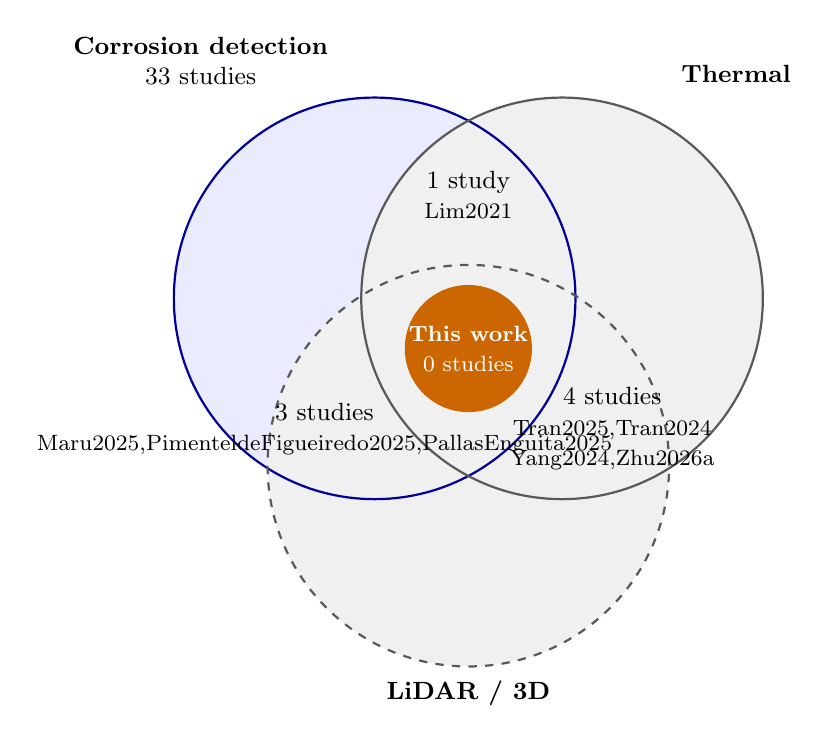
\begin{tikzpicture}[scale=0.85, every node/.style={font=\small, align=center}]
  \fill[blue!8]  (-1.4,0.9) circle (3);
  \fill[gray!12] (1.4,0.9)  circle (3);
  \fill[gray!12] (0,-1.6)   circle (3);
  \draw[thick, blue!60!black] (-1.4,0.9) circle (3);
  \draw[thick, gray!70!black] (1.4,0.9)  circle (3);
  \draw[thick, gray!70!black, dashed] (0,-1.6) circle (3);
  \node at (-4.0,4.45) {\textbf{Corrosion detection}\\33 studies};
  \node at (4.0,4.25)  {\textbf{Thermal}};
  \node at (0,-5.0)    {\textbf{LiDAR / 3D}};
  \node at (0,2.45)    {1 study\\ \footnotesize \citep{Lim2021}};
  \node at (-2.15,-1.05) {3 studies\\ \footnotesize \citep{Maru2025,PimenteldeFigueiredo2025,PallasEnguita2025}};
  \node at (2.15,-1.05)  {4 studies\\ \footnotesize \citep{Tran2025,Tran2024}\\ \footnotesize \citep{Yang2024,Zhu2026a}};
  \fill[orange!80!black] (0,0.15) circle (0.95);
  \node[text=white] at (0,0.15) {\footnotesize\textbf{This work}\\ \footnotesize 0 studies};
\end{tikzpicture}
\caption[Overlap of the reviewed studies]{Overlap of the reviewed studies on corrosion detection, thermal sensing
and LiDAR or 3D sensing; no study lies in the center}
\label{fig:gap}
\end{figure}

Table~\ref{tab:closest} compares this work with the closest studies. Each covers
part of the problem. An RGB-only YOLO detector identifies metal surface corrosion
but uses one sensor \citep{Fu2024}. RGB-thermal fusion detects corrosion on steel bridges
but has no geometry \citep{Lim2021}. RGB-LiDAR fusion measures metal loss, but only on
laboratory plates and without thermal data \citep{Maru2025}. RGB with laser triangulation
tests the value of geometric data for corrosion but has no thermal data and no
measurement of metal loss \citep{Haitz2022}. The MID-1K study senses RGB, thermal and
LiDAR and compares single sensors with their fusion, but detects people rather
than corrosion \citep{Mota2024}.

\begin{table}[htbp]
\centering
\caption{This work compared with the closest reviewed studies}
\label{tab:closest}
\footnotesize
\renewcommand{\arraystretch}{1.2}
\setlength{\tabcolsep}{4pt}
\begin{tabularx}{\textwidth}{@{}>{\RaggedRight\arraybackslash}X*{6}{>{\centering\arraybackslash}p{1.65cm}}@{}}
\toprule
\textbf{Study} & \textbf{RGB} & \textbf{Thermal} & \textbf{LiDAR or 3D} & \textbf{Corrosion} & \textbf{Metal loss} & \textbf{Tests each sensor} \\
\midrule
Fu et al.\ (2024), RGB + YOLO \citep{Fu2024} & \cmY & \cmN & \cmN & \cmY & \cmN & \cmN \\
Lim et al.\ (2021), RGB + thermal \citep{Lim2021} & \cmY & \cmY & \cmN & \cmY & \cmN & \cmY \\
Maru et al.\ (2025), RGB + LiDAR, laboratory \citep{Maru2025} & \cmY & \cmN & \cmY & \cmY & \cmY & \cmY \\
Haitz et al.\ (2022), RGB + laser triangulation \citep{Haitz2022} & \cmY & \cmN & \cmY & \cmY & \cmN & \cmY \\
Mota et al.\ (2024), RGB + thermal + LiDAR, people \citep{Mota2024} & \cmY & \cmY & \cmY & \cmN & \cmN & \cmY \\
\midrule
\textbf{This work} & \cmY & \cmY & \cmY & \cmY & \cmY & \cmY \\
\bottomrule
\end{tabularx}

\vspace{2pt}
\raggedright\footnotesize\textit{Note.} \citet{Haitz2022} and \citet{Mota2024} are
conference papers, included because no journal study in the review reports the
same comparison.
\end{table}

The review therefore identifies three gaps.
\begin{enumerate}[label=(\roman*)]
  \item \textbf{Sensors.} No reviewed corrosion study fuses RGB, thermal and
        LiDAR data. Of the 33 corrosion-sensing studies, 16 rely on RGB images
        alone, and the one study that adds thermal imaging heats the steel with
        lamps and has no geometric data \citep{Lim2021}. The only studies that combine
        all three sensors address driving or calibration \citep{Tran2025,Tran2024,Yang2024}.
  \item \textbf{Measurement.} Metal loss is measured by contact or on laboratory
        specimens \citep{Huang2026a,Egodawela2025,Khodabux2021a,Maru2025,Zheng2025}, and severity is reported in
        incompatible ways, if at all. No reviewed study estimates both the area
        and the metal loss of detected corrosion from contactless data.
  \item \textbf{Evidence.} An added sensor does not always help \citep{Jiang2024,Tran2025}, and
        nine fusion studies name alignment as a limitation. What each of RGB,
        thermal and LiDAR contributes to corrosion detection has not been
        measured under controlled conditions.
\end{enumerate}

This research addresses these gaps by registering RGB, thermal and LiDAR data of
corroded metal surfaces into a common frame, detecting corroded regions with an
early-fusion YOLO detector that also estimates the area and metal loss of each
region from the LiDAR, and measuring the contribution of each sensor through a
controlled ablation. The methodology is described in Chapter~\ref{ch:methodology}.
